% DO NOT COMPILE THIS FILE DIRECTLY!
% This is included by the other .tex files.

\lstdefinelanguage{json}{
    basicstyle=\ttfamily\footnotesize,
    numbers=left,
    numberstyle=\ttfamily\footnotesize,
    stepnumber=1,
    numbersep=8pt,
    showstringspaces=false,
    breaklines=true,
    frame=lines,
    title=\lstname,
    backgroundcolor=\color{background},
    literate=
     *{0}{{{\color{numb}0}}}{1}
      {1}{{{\color{numb}1}}}{1}
      {2}{{{\color{numb}2}}}{1}
      {3}{{{\color{numb}3}}}{1}
      {4}{{{\color{numb}4}}}{1}
      {5}{{{\color{numb}5}}}{1}
      {6}{{{\color{numb}6}}}{1}
      {7}{{{\color{numb}7}}}{1}
      {8}{{{\color{numb}8}}}{1}
      {9}{{{\color{numb}9}}}{1}
      {:}{{{\color{punct}{:}}}}{1}
      {,}{{{\color{punct}{,}}}}{1}
      {\{}{{{\color{delim}{\{}}}}{1}
      {\}}{{{\color{delim}{\}}}}}{1}
      {[}{{{\color{delim}{[}}}}{1}
      {]}{{{\color{delim}{]}}}}{1},
}

\begin{frame}[t,plain]
\titlepage
\end{frame}

\begin{frame}[fragile]
        \frametitle{Why we want to go more modular...}
        \begin{itemize}
        \item Ways to extend MISP before modules
            \begin{itemize}
            \item APIs (PyMISP, MISP API)
                \begin{itemize}
                    \item Works really well
                    \item {\bf No integration with the UI}
                \end{itemize}
            \item Change the core code
                \begin{itemize}
                    \item Have to change the core of MISP, diverge from upstream
                    \item Needs a deep understanding of MISP internals
                    \item Let's not beat around the bush: {\bf Everyone hates PHP}
                \end{itemize}
            \end{itemize}
        \end{itemize}
\end{frame}

\begin{frame}[fragile]
        \frametitle{Goals for the module system}
        \begin{itemize}
        \item Have a way to extend MISP without altering the core
        \item Get started {\bf quickly} without a need to study the internals
        \item Make the {\bf modules as light weight as possible}
            \begin{itemize}
                \item Module developers should only have to worry about the data transformation
                \item Modules should have a simple and clean skeleton
            \end{itemize}
        \item In a friendlier language - {\bf Python}
        \end{itemize}
\end{frame}

\begin{frame}
        \frametitle{MISP modules - extending MISP with Python scripts}
        \begin{columns}[t]
        \column{5.6cm}
        \begin{figure}
        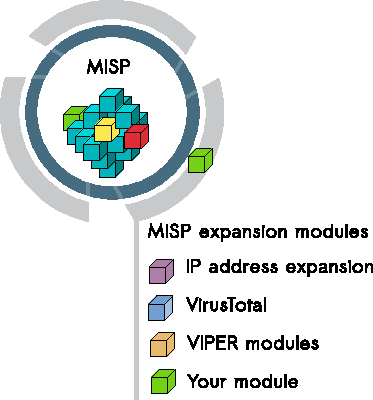
\includegraphics[scale=0.70]{misp-expansion.pdf}
        \end{figure}
        \column{6.4cm}
        \begin{itemize}
                \item Extending MISP with expansion modules with zero customization in MISP.
                \item A simple ReST API between the modules and MISP allowing auto-discovery of new modules with their features.
                \item Benefit from existing Python modules in Viper or any other tools.
                \item MISP modules functionnality introduced in MISP 2.4.28.
                \item MISP import/export modules introduced in MISP 2.4.50.
        \end{itemize}
         \end{columns}
\end{frame}

\begin{frame}[fragile]
        \frametitle{MISP modules - installation}
        \begin{itemize}
        \item MISP modules can be run on the same system or on a remote server.
        \item Python 3 is required to run MISP modules.
            \begin{itemize}
                \item sudo apt-get install python3-dev python3-pip libpq5
                \item cd /usr/local/src/
                \item sudo git clone https://github.com/MISP/misp-modules.git
                \item cd misp-modules
                \item sudo pip3 install -I -r REQUIREMENTS
                \item sudo pip3 install -I .
                \item sudo vi /etc/rc.local, add this line: `sudo -u www-data misp-modules -s \&`
            \end{itemize}
        \end{itemize}

\end{frame}

\begin{frame}
        \frametitle{MISP modules - Simple REST API mechanism}
        \begin{itemize}
                \item http://127.0.0.1:6666/modules - introspection interface to get {\bf all modules available}
                        \begin{itemize}
                                \item returns a JSON with a description of each module
                        \end{itemize}
                \item http://127.0.0.1:6666/query - interface to {\bf query a specific module}
                        \begin{itemize}
                                \item to send a JSON to query the module
                        \end{itemize}
                \item {\bf MISP autodiscovers} the available modules and the MISP site administrator can enable modules as they wish.
                \item If a configuration is required for a module, {\bf MISP adds automatically the option} in the server settings.
        \end{itemize}
\end{frame}

\begin{frame}[fragile]
        \frametitle{Finding available MISP modules}
        \begin{itemize}
                \item curl -s http://127.0.0.1:6666/modules | jq .
        \end{itemize}
        \begin{adjustbox}{width=\textwidth,height=6cm,keepaspectratio}
        \begin{lstlisting}[language=json,firstnumber=1]
            {
            "type": "expansion",
            "name": "dns",
            "meta": {
              "module-type": [
                "expansion",
                "hover"
              ],
              "description": "Simple DNS expansion service to resolve IP address from MISP attributes",
              "author": "Alexandre Dulaunoy",
              "version": "0.1"
            },
            "mispattributes": {
              "output": [
                "ip-src",
                "ip-dst"
              ],
              "input": [
                "hostname",
                "domain"
              ]
            }
        \end{lstlisting}
        \end{adjustbox}
\end{frame}

\begin{frame}
        \frametitle{MISP modules - configuration in the UI}
        \includegraphics[scale=0.50]{modules-integration.png}
\end{frame}

\begin{frame}
        \frametitle{MISP modules - How it's integrated in the UI?}
        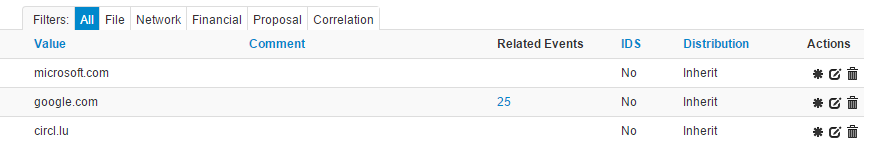
\includegraphics[scale=0.40]{screenshots/enrichment1.PNG}\\
        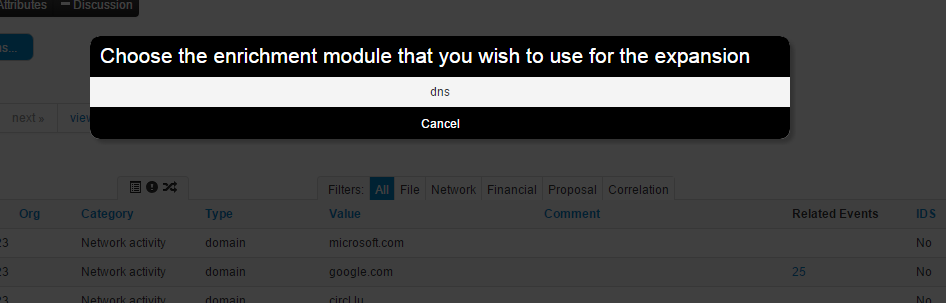
\includegraphics[scale=0.38]{screenshots/enrichment2.PNG}\\
        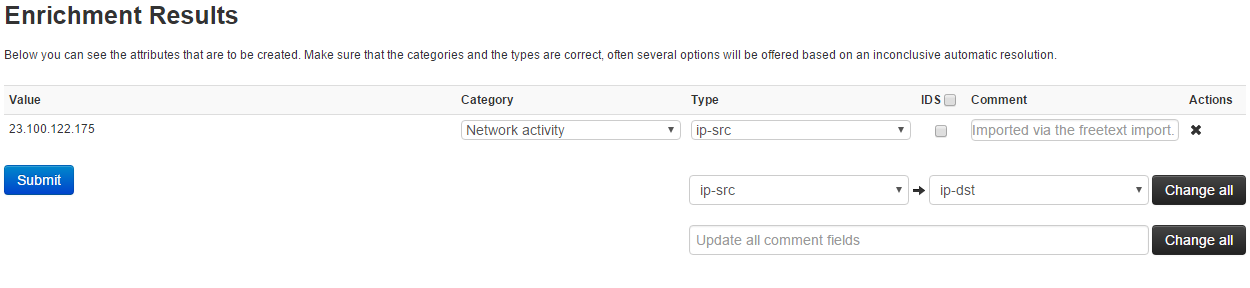
\includegraphics[scale=0.35]{screenshots/enrichment3.PNG}
\end{frame}

\begin{frame}
        \frametitle{MISP modules - main types of modules}
        \begin{itemize}
            \item Expansion modules - enrich data that is in MISP
                    \begin{itemize}
                        \item Hover type - showing the expanded values directly on the attributes
                        \item Expansion type - showing and adding the expanded values via a proposal form
                    \end{itemize}
            \item Import modules - import new data into MISP
            \item Export modules - export existing data from MISP
        \end{itemize}
\end{frame}

% \begin{frame}[fragile]
%       \frametitle{Creating your Expansion module (Skeleton)}
%       \begin{adjustbox}{width=\textwidth,height=5cm,keepaspectratio}
%       \begin{lstlisting}[language=python]
%         import json
%         import dns.resolver
%
%         misperrors = {'error' : 'Error'}
%         mispattributes = {'input': [], 'output': []}
%         moduleinfo = {'version': '', 'author': '',
%                       'description': '', 'module-type': []}
%
%         def handler(q=False):
%             if q is False:
%                 return False
%             request = json.loads(q)
%             r = {'results': [{'types': [], 'values':[]}]}
%             return r
%         def introspection():
%             return mispattributes
%         def version():
%             return moduleinfo
%
%               \end{lstlisting}
%         \end{adjustbox}
% \end{frame}

% \begin{frame}[fragile]
%       \frametitle{Creating your Expansion module (metadata 1)}
%       \begin{adjustbox}{width=\textwidth,height=5cm,keepaspectratio}
%       \begin{lstlisting}[language=python]
%         misperrors = {'error' : 'Error'}
%         mispattributes = {'input': ['hostname', 'domain'], 'output': ['ip-src', 'ip-dst']}
%         moduleinfo = {'version': '', 'author': '',
%                       'description': '', 'module-type': []}
%               \end{lstlisting}
%         \end{adjustbox}
% \end{frame}
%
% \begin{frame}[fragile]
%       \frametitle{Creating your Expansion module (metadata 2)}
%       \begin{adjustbox}{width=\textwidth,height=10cm,keepaspectratio}
%       \begin{lstlisting}[language=python,showstringspaces=false]
%         misperrors = {'error' : 'Error'}
%         mispattributes = {'input': ['hostname', 'domain'], 'output': ['ip-src', 'ip-dst']}
%         moduleinfo = {'version': '0.1', 'author': 'Alexandre Dulaunoy',
%                      'description': 'Simple DNS expansion service to
%               resolve IP address from MISP attributes', 'module-type': ['expansion','hover']}
%         \end{lstlisting}
%         \end{adjustbox}
% \end{frame}
%
% \begin{frame}[fragile]
%       \frametitle{Creating your Expansion module (handler 1)}
%       \begin{adjustbox}{width=\textwidth,height=5cm,keepaspectratio}
%       \begin{lstlisting}[language=python]
%         def handler(q=False):
%             if q is False:
%                 return False
%             request = json.loads(q)
%             # MAGIC
%             # MORE MAGIC
%             r = {'results': [
%                 {'types': output_types, 'values':values},
%                 {'types': output_types2, 'values':values2}
%             ]}
%             return r
%               \end{lstlisting}
%         \end{adjustbox}
% \end{frame}
%
%
% \begin{frame}[fragile]
%       \frametitle{Creating your Expansion module (handler 2)}
%       \begin{adjustbox}{width=\textwidth,height=5cm,keepaspectratio}
%       \begin{lstlisting}[language=python]
%             if request.get('hostname'):
%                 toquery = request['hostname']
%             elif request.get('domain'):
%                 toquery = request['domain']
%             else:
%                 return False
%             r = dns.resolver.Resolver()
%             r.timeout = 2
%             r.lifetime = 2
%             r.nameservers = ['8.8.8.8']
%             try:
%                 answer = r.query(toquery, 'A')
%             except dns.resolver.NXDOMAIN:
%                 misperrors['error'] = "NXDOMAIN"
%                 return misperrors
%             except dns.exception.Timeout:
%                 misperrors['error'] = "Timeout"
%                 return misperrors
%             except:
%                 misperrors['error'] = "DNS resolving error"
%                 return misperrors
%             r = {'results': [{'types': mispattributes['output'], 'values':[str(answer[0])]}]}
%             return r
%               \end{lstlisting}
%         \end{adjustbox}
% \end{frame}

\begin{frame}[fragile]
        \frametitle{Querying a module}
        \begin{itemize}
                \item curl -s http://127.0.0.1:6666/query -H "Content-Type: application/json" --data @body.json -X POST
        \end{itemize}
        \begin{lstlisting}[language=json,firstnumber=1]{body.json}
        {"module": "dns", "hostname": "www.circl.lu"}
        \end{lstlisting}
        \begin{itemize}
                \item and the response of the dns module:
        \end{itemize}
        \begin{lstlisting}[language=json,firstnumber=1]
        {"results": [{"values": ["149.13.33.14"],
         "types": ["ip-src", "ip-dst"]}]}
        \end{lstlisting}
\end{frame}

 \begin{frame}[fragile]
      \frametitle{Creating your module - DNS module}
      \begin{adjustbox}{width=\textwidth,height=5cm,keepaspectratio}
      \begin{lstlisting}[language=python]
        import json
        import dns.resolver
        misperrors = {'error': 'Error'}
        mispattributes = {'input': ['hostname', 'domain', 'domain|ip'], 'output': ['ip-src','ip-dst']}
        moduleinfo = {'version': '0.3', 'author': 'Alexandre Dulaunoy','description': 'Simple DNS expansion service to resolve IP address from MISP attributes',
                    'module-type': ['expansion', 'hover']}
        moduleconfig = ['nameserver']

        def handler(q=False):
            if q is False:
                return False
            request = json.loads(q)
            if request.get('hostname'):
                toquery = request['hostname']
            elif request.get('domain'):
                toquery = request['domain']
            elif request.get('domain|ip'):
                toquery = request['domain|ip'].split('|')[0]
            else:
                return False
            r = dns.resolver.Resolver()
            r.timeout = 2
            r.lifetime = 2

            if request.get('config'):
                if request['config'].get('nameserver'):
                    nameservers = []
                    nameservers.append(request['config'].get('nameserver'))
                    r.nameservers = nameservers
            else:
                r.nameservers = ['8.8.8.8']

            try:
                answer = r.resolve(toquery, 'A')
            except dns.resolver.NXDOMAIN:
                misperrors['error'] = "NXDOMAIN"
                return misperrors
            except ...

            return {'results': [{'types': mispattributes['output'], 'values':[str(answer[0])]}]}

        def introspection():
            return mispattributes

        def version():
            moduleinfo['config'] = moduleconfig
            return moduleinfo
        \end{lstlisting}
        \end{adjustbox}
\end{frame}

\begin{frame}[t,fragile]
        \frametitle{Testing your module}
        \begin{itemize}
                \item Copy your module dns.py in modules/expansion/
                \item Restart the server misp-modules.py
        \end{itemize}
        \begin{adjustbox}{width=\textwidth,height=5cm,keepaspectratio}
        \begin{lstlisting}
        [adulau:~/git/misp-modules/bin]$ python3 misp-modules.py
        2016-03-20 19:25:43,748 - misp-modules - INFO - MISP modules passivetotal imported
        2016-03-20 19:25:43,787 - misp-modules - INFO - MISP modules sourcecache imported
        2016-03-20 19:25:43,789 - misp-modules - INFO - MISP modules cve imported
        2016-03-20 19:25:43,790 - misp-modules - INFO - MISP modules dns imported
        2016-03-20 19:25:43,797 - misp-modules - INFO - MISP modules server started on TCP port 6666
        \end{lstlisting}
        \end{adjustbox}
        \begin{itemize}
                \item Check if your module is present in the introspection
                \item curl -s http://127.0.0.1:6666/modules
                \item If yes, test it directly with MISP or via curl
        \end{itemize}
\end{frame}

\begin{frame}[fragile]
    \frametitle{Code samples (Configuration)}
    \begin{adjustbox}{width=\textwidth,height=5cm,keepaspectratio}
        \begin{lstlisting}[language=python]
            # Configuration at the top
            moduleconfig = ['username', 'password']

            # Code block in the handler
            if not request.get('config'):
                return {'error': 'CIRCL Passive SSL authentication is missing.'}

            if not request['config'].get('username') or not request['config'].get('password'):
                return {'error': 'CIRCL Passive SSL authentication is incomplete, please provide your username and password.'}
            authentication = (request['config']['username'], request['config']['password'])

            if not request.get('attribute') or not check_input_attribute(request['attribute']):
                return {'error': f'{standard_error_message}, which should contain at least a type, a value and an uuid.'}
            attribute = request['attribute']
-
            pssl_parser = PassiveSSLParser(attribute, authentication)

          \end{lstlisting}
    \end{adjustbox}
\end{frame}

\begin{frame}[fragile]
        \frametitle{Default expansion module set}
        \begin{itemize}
                \item asn history
                \item CIRCL Passive DNS
                \item CIRCL Passive SSL
                \item Country code lookup
                \item CVE information expansion
                \item DNS resolver
                \item DomainTools
                \item eupi (checking url in phishing database)
                \item ipasn
                \item PassiveTotal - http://blog.passivetotal.org/misp-sharing-done-differently
                \item sourcecache
                \item Virustotal
                \item Whois
                \item ...
        \end{itemize}
\end{frame}

\begin{frame}[fragile]
        \frametitle{Import modules}
        \begin{itemize}
            \item Similar to expansion modules
            \item Input is a file upload or a text paste
            \item Output is a list of parsed attributes to be editend and verified by the user
            \item Some examples
            \begin{itemize}
                \item Cuckoo JSON import
                \item email import
                \item OCR module
                \item Open IoC import
            \end{itemize}
       \end{itemize}
\end{frame}

% \begin{frame}[fragile]
%       \frametitle{Creating your Import module (Skeleton)}
%       \begin{adjustbox}{width=\textwidth,height=5cm,keepaspectratio}
%       \begin{lstlisting}[language=python]
%         import json
%
%         misperrors = {'error' : 'Error'}
%         userConfig = {
%                          'number1': {
%                              'type': 'Integer',
%                              'regex': '/^[0-4]$/i',
%                              'errorMessage': 'Expected a number in range [0-4]',
%                              'message': 'Column number used for value'
%                          }
%                      };
%         inputSource = ['file', 'paste']
%         moduleinfo = {'version': '', 'author': '',
%                       'description': '', 'module-type': ['import']}
%         moduleconfig=[]
%
%         def handler(q=False):
%             if q is False:
%                 return False
%             request = json.loads(q)
%             request["data"] = base64.b64decode(request["data"])
%             r = {'results': [{'categories': [], 'types': [], 'values':[]}]}
%             return r
%
%         def introspection():
%             return {'userConfig': userConfig, 'inputSource': inputSource, 'moduleConfig': moduleConfig}
%
%         def version():
%             return moduleinfo
%               \end{lstlisting}
%         \end{adjustbox}
% \end{frame}

% \begin{frame}[fragile]
%     \frametitle{Creating your import module (userConfig and inputSource)}
%     \begin{adjustbox}{width=\textwidth,height=5cm,keepaspectratio}
%         \begin{lstlisting}[language=python]
%             userConfig = {
%                 'number1': {
%                     'type': 'Integer',
%                     'regex': '/^[0-4]$/i',
%                     'errorMessage': 'Expected a number in range [0-4]',
%                     'message': 'Column number used for value'
%                 }
%             };
%             inputSource = ['file', 'paste']
%         \end{lstlisting}
%     \end{adjustbox}
% \end{frame}
%
% \begin{frame}[fragile]
%     \frametitle{Creating your import module (Handler)}
%     \begin{adjustbox}{width=\textwidth,height=5cm,keepaspectratio}
%         \begin{lstlisting}[language=python]
%             def handler(q=False):
%                 if q is False:
%                     return False
%                 request = json.loads(q)
%                 request["data"] = base64.b64decode(request["data"])
%                 r = {'results': [{'categories': [], 'types': [], 'values':[]}]}
%                 return r
%         \end{lstlisting}
%     \end{adjustbox}
% \end{frame}
%
% \begin{frame}[fragile]
%     \frametitle{Creating your import module (Introspection)}
%     \begin{adjustbox}{width=\textwidth,height=5cm,keepaspectratio}
%         \begin{lstlisting}[language=python]
%             def introspection():
%                 modulesetup = {}
%                 try:
%                     userConfig
%                     modulesetup['userConfig'] = userConfig
%                 except NameError:
%                     pass
%                 try:
%                     moduleConfig
%                     modulesetup['moduleConfig'] = moduleConfig
%                 except NameError:
%                     pass
%                 try:
%                     inputSource
%                     modulesetup['inputSource'] = inputSource
%                 except NameError:
%                     pass
%                 return modulesetup
%         \end{lstlisting}
%     \end{adjustbox}
% \end{frame}

\begin{frame}[fragile]
    \frametitle{Export modules}
    \begin{itemize}
        \item Not the preferred way to export data from MISP
        \item Input is currently only a single event
        \item Output is a file in the export format served back to the user
        \item Will be moved / merged with MISP built-in export modules
        \begin{itemize}
            \item Allows export of event / attribute collections
        \end{itemize}
    \end{itemize}
\end{frame}

% \begin{frame}[fragile]
%       \frametitle{Creating your Export module (Skeleton)}
%       \begin{adjustbox}{width=\textwidth,height=5cm,keepaspectratio}
%       \begin{lstlisting}[language=python]
%         import json
%         inputSource = ['event']
%         outputFileExtension = 'txt'
%         responseType = 'application/txt'
%         moduleinfo = {'version': '0.1', 'author': 'Andras Iklody',
%                       'description': 'Skeleton export module',
%                       'module-type': ['export']}
%
%         def handler(q=False):
%             if q is False:
%                 return False
%             request = json.loads(q)
%             # insert your magic here!
%             output = my_magic(request["data"])
%             r = {"data":base64.b64encode(output.encode('utf-8')).decode('utf-8')}
%             return r
%
%         def introspection():
%             return {'userConfig': userConfig, 'inputSource': inputSource, 'moduleConfig': moduleConfig, 'outputFileExtension': outputFileExtension}
%
%         def version():
%             return moduleinfo
%               \end{lstlisting}
%         \end{adjustbox}
% \end{frame}
%
% \begin{frame}[fragile]
%     \frametitle{Creating your export module (settings)}
%     \begin{adjustbox}{width=\textwidth,height=5cm,keepaspectratio}
%         \begin{lstlisting}[language=python]
%             inputSource = ['event']
%             outputFileExtension = 'txt'
%             responseType = 'application/txt'
%         \end{lstlisting}
%     \end{adjustbox}
% \end{frame}
%
% \begin{frame}[fragile]
%     \frametitle{Creating your export module (handler)}
%     \begin{adjustbox}{width=\textwidth,height=5cm,keepaspectratio}
%         \begin{lstlisting}[language=python]
%             def handler(q=False):
%                 if q is False:
%                     return False
%                 request = json.loads(q)
%                 # insert your magic here!
%                 output = my_magic(request["data"])
%                 r = {"data":base64.b64encode(output.encode('utf-8')).decode('utf-8')}
%                 return r
%         \end{lstlisting}
%     \end{adjustbox}
% \end{frame}
%
% \begin{frame}[fragile]
%     \frametitle{Creating your export module (introspection)}
%     \begin{adjustbox}{width=\textwidth,height=5cm,keepaspectratio}
%         \begin{lstlisting}[language=python]
%             def introspection():
%                 modulesetup = {}
%                 try:
%                     responseType
%                     modulesetup['responseType'] = responseType
%                 except NameError:
%                     pass
%                 try:
%                     userConfig
%                     modulesetup['userConfig'] = userConfig
%                 except NameError:
%                     pass
%                 try:
%                     moduleConfig
%                     modulesetup['moduleConfig'] = moduleConfig
%                 except NameError:
%                     pass
%                 try:
%                     outputFileExtension
%                     modulesetup['outputFileExtension'] = outputFileExtension
%                 except NameError:
%                     pass
%                 try:
%                     inputSource
%                     modulesetup['inputSource'] = inputSource
%                 except NameError:
%                     pass
%                 return modulesetup
%         \end{lstlisting}
%     \end{adjustbox}
% \end{frame}

\begin{frame}[fragile]
    \frametitle{New expansion \& import modules format}
    \begin{itemize}
        \item Backward compatible - an additional field to extend the format
    \end{itemize}
    \begin{adjustbox}{width=\textwidth,height=5cm,keepaspectratio}
        \begin{lstlisting}[language=python]
            misp_attributes = {'input': [...], 'output': [...],
                               'format': 'misp_standard'}
        \end{lstlisting}
    \end{adjustbox}
    \begin{itemize}
        \item Takes a standard MISP attribute as input
        \item Returns MISP format
        \begin{itemize}
            \item Attributes
            \item Objects (with their references)
            \item Tags
        \end{itemize}
    \end{itemize}
    \begin{adjustbox}{width=\textwidth,height=5cm,keepaspectratio}
        \begin{lstlisting}[language=python]
            results = {'Attribute': [...], 'Object': [...],
                       'Tag': [...]}
        \end{lstlisting}
    \end{adjustbox}
    \begin{itemize}
        \item First modules supporting this new export format
            \begin{itemize}
                \item urlhaus expansion module
                \item Joe Sandbox import \& query module
            \end{itemize}
    \end{itemize}
\end{frame}

\begin{frame}[fragile]
        \frametitle{New expansion \& import modules view (MISP 2.4.110)}
    \includegraphics[scale=0.2]{new_format_view.png}
\end{frame}


\begin{frame}[fragile]
    \frametitle{New - Standalone Functionality}
    \begin{itemize}
        \item Flexibility, no need to install MISP
        \item User friendly interface
        \item Easiest way to test new modules
    \end{itemize}
\end{frame}

\begin{frame}[fragile]
    \frametitle{Web interface - Query}
    \begin{itemize}
        \item Add multiple entries
        \item Choose different modules
    \end{itemize}
    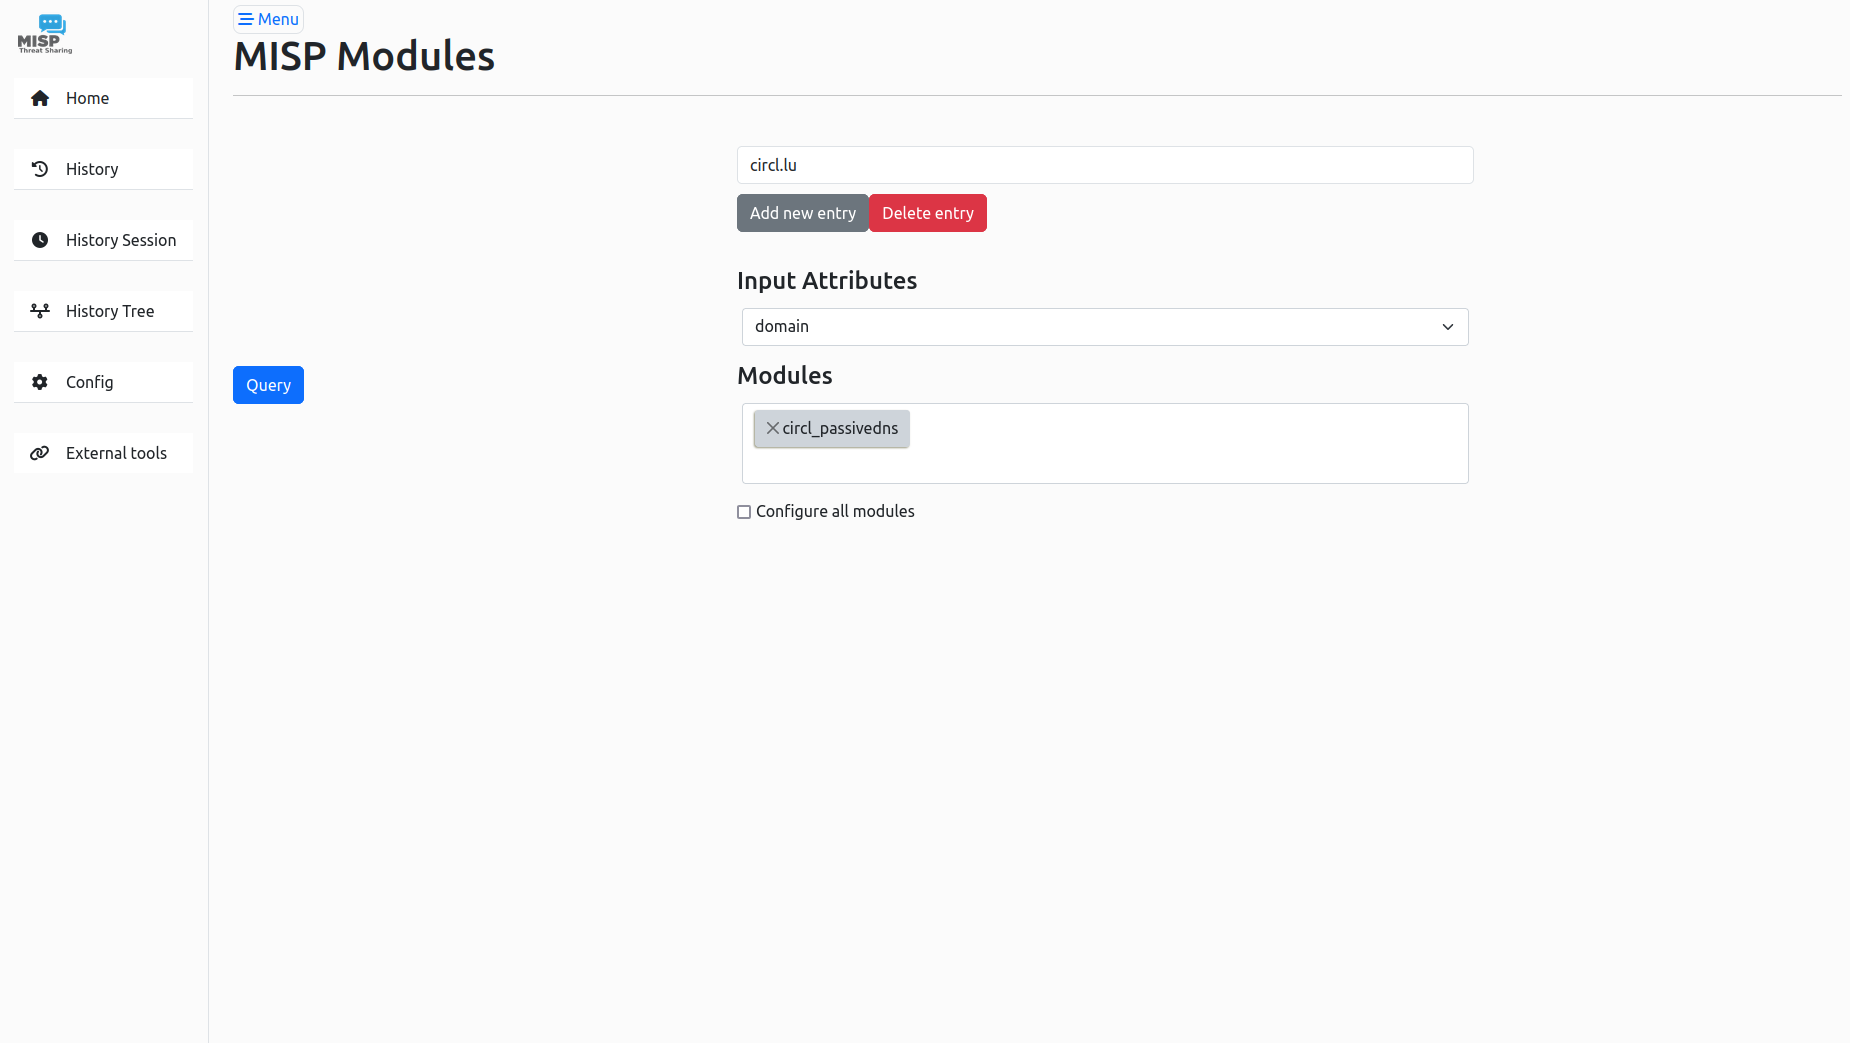
\includegraphics[scale=0.23]{screenshots/misp_module_index.png}
\end{frame}

\begin{frame}[fragile]
    \frametitle{Web interface - Results}
    \begin{itemize}
        \item Multiple tabs for visualization in different formats
    \end{itemize}
    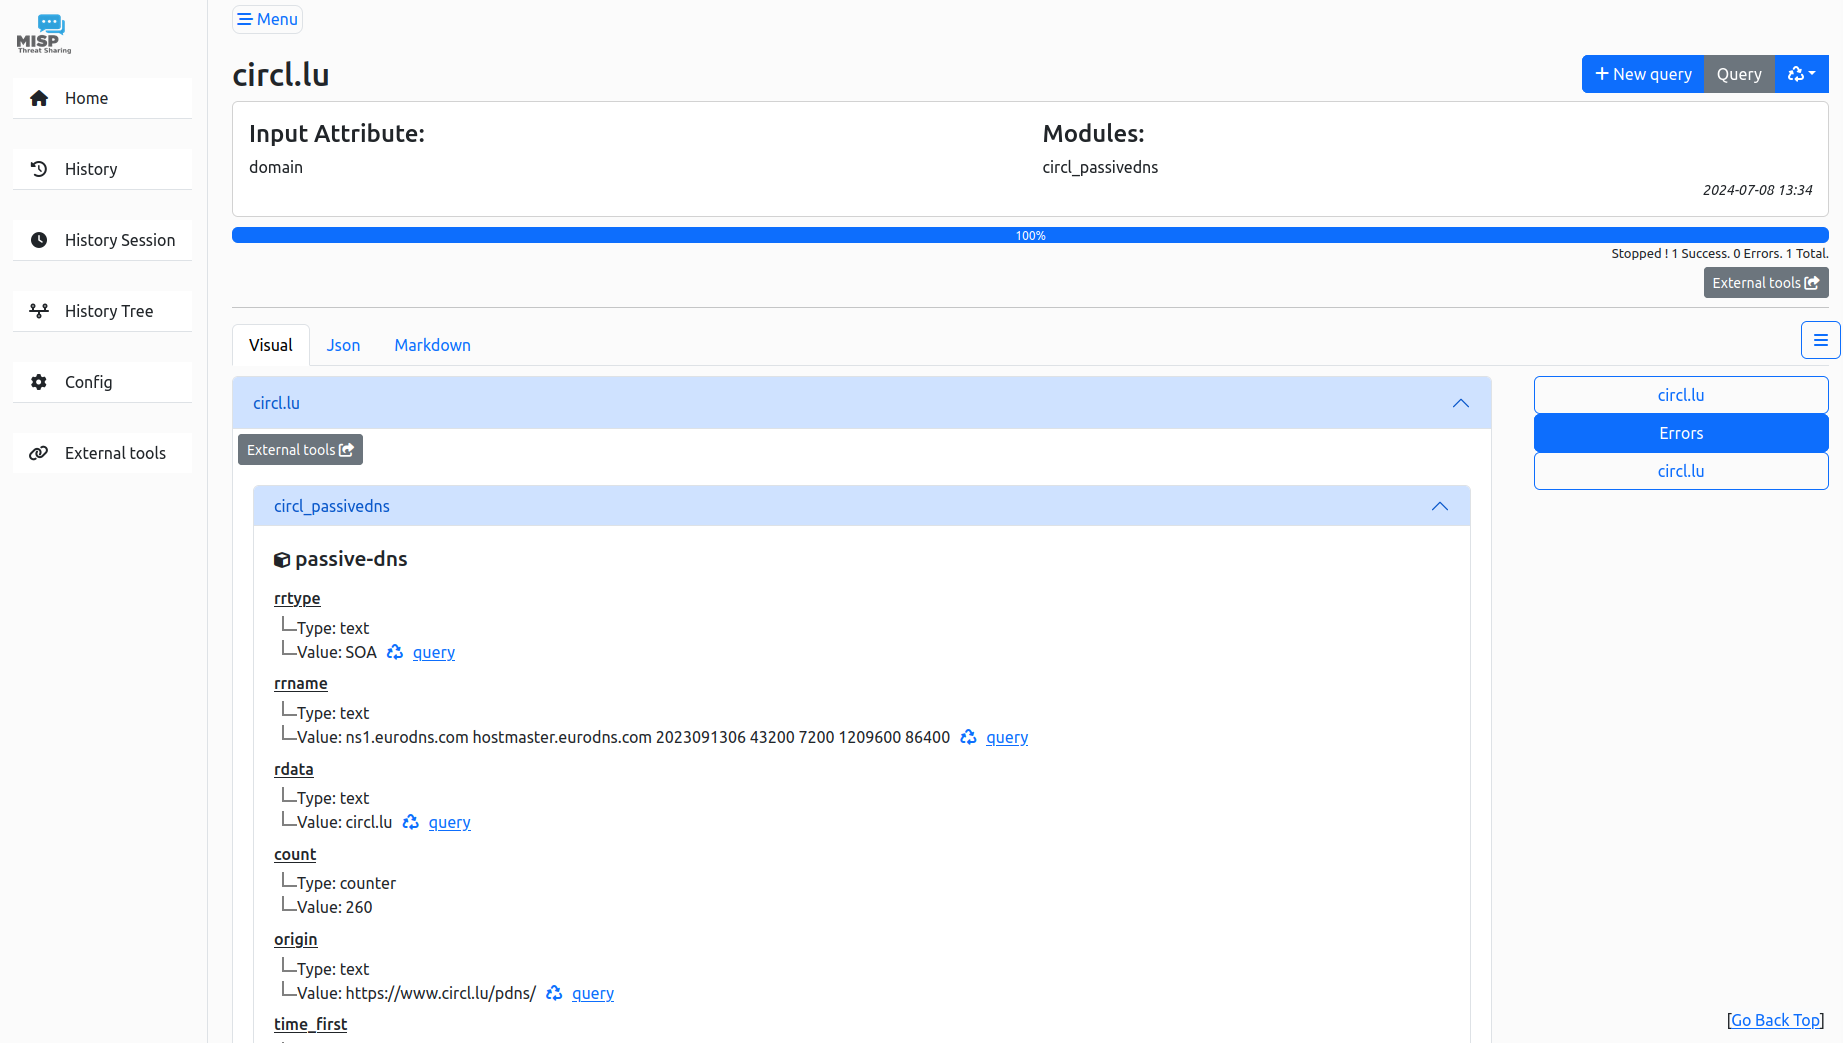
\includegraphics[scale=0.23]{screenshots/misp_module_results.png}
\end{frame}

\begin{frame}[fragile]
    \frametitle{Web interface - History}
    \begin{itemize}
        \item Save your researches and pivot from them
    \end{itemize}
    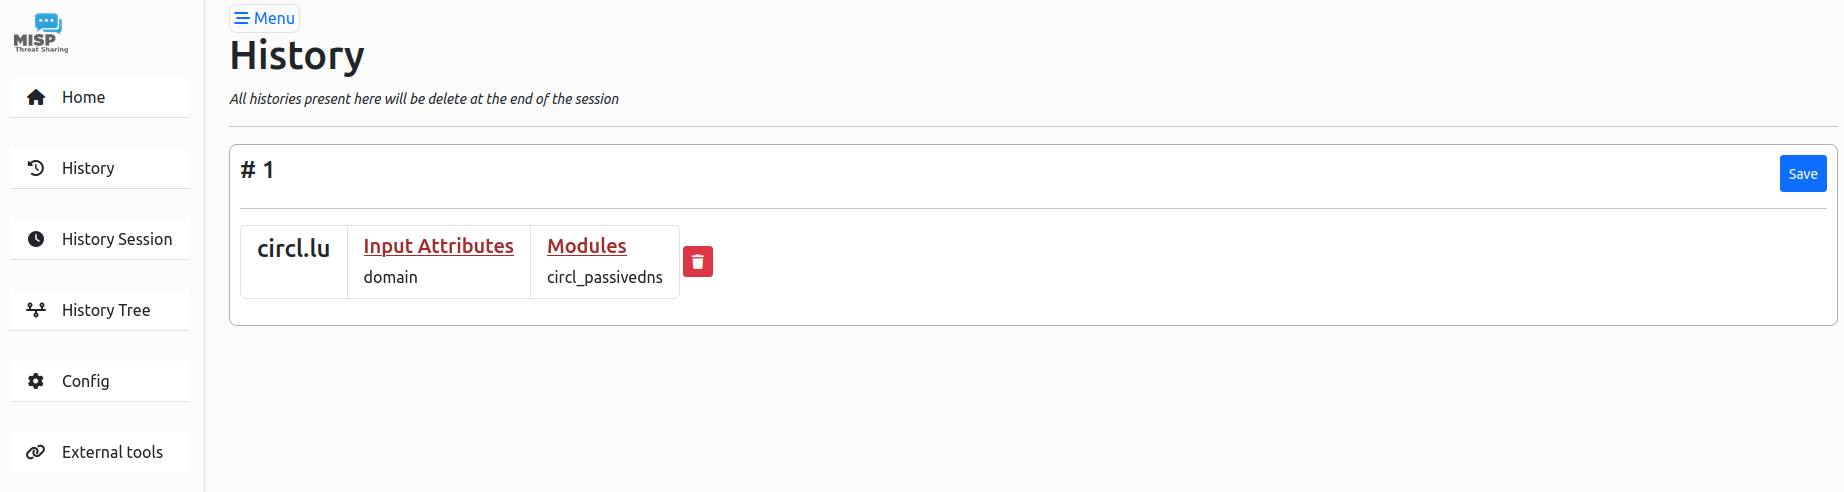
\includegraphics[scale=0.23]{screenshots/misp_module_history.png}
\end{frame}

\begin{frame}[fragile]
    \begin{itemize}
        \item Export results to other tools. (Still in dev)
    \end{itemize}
    \frametitle{Web interface - External tools (Dev)}
    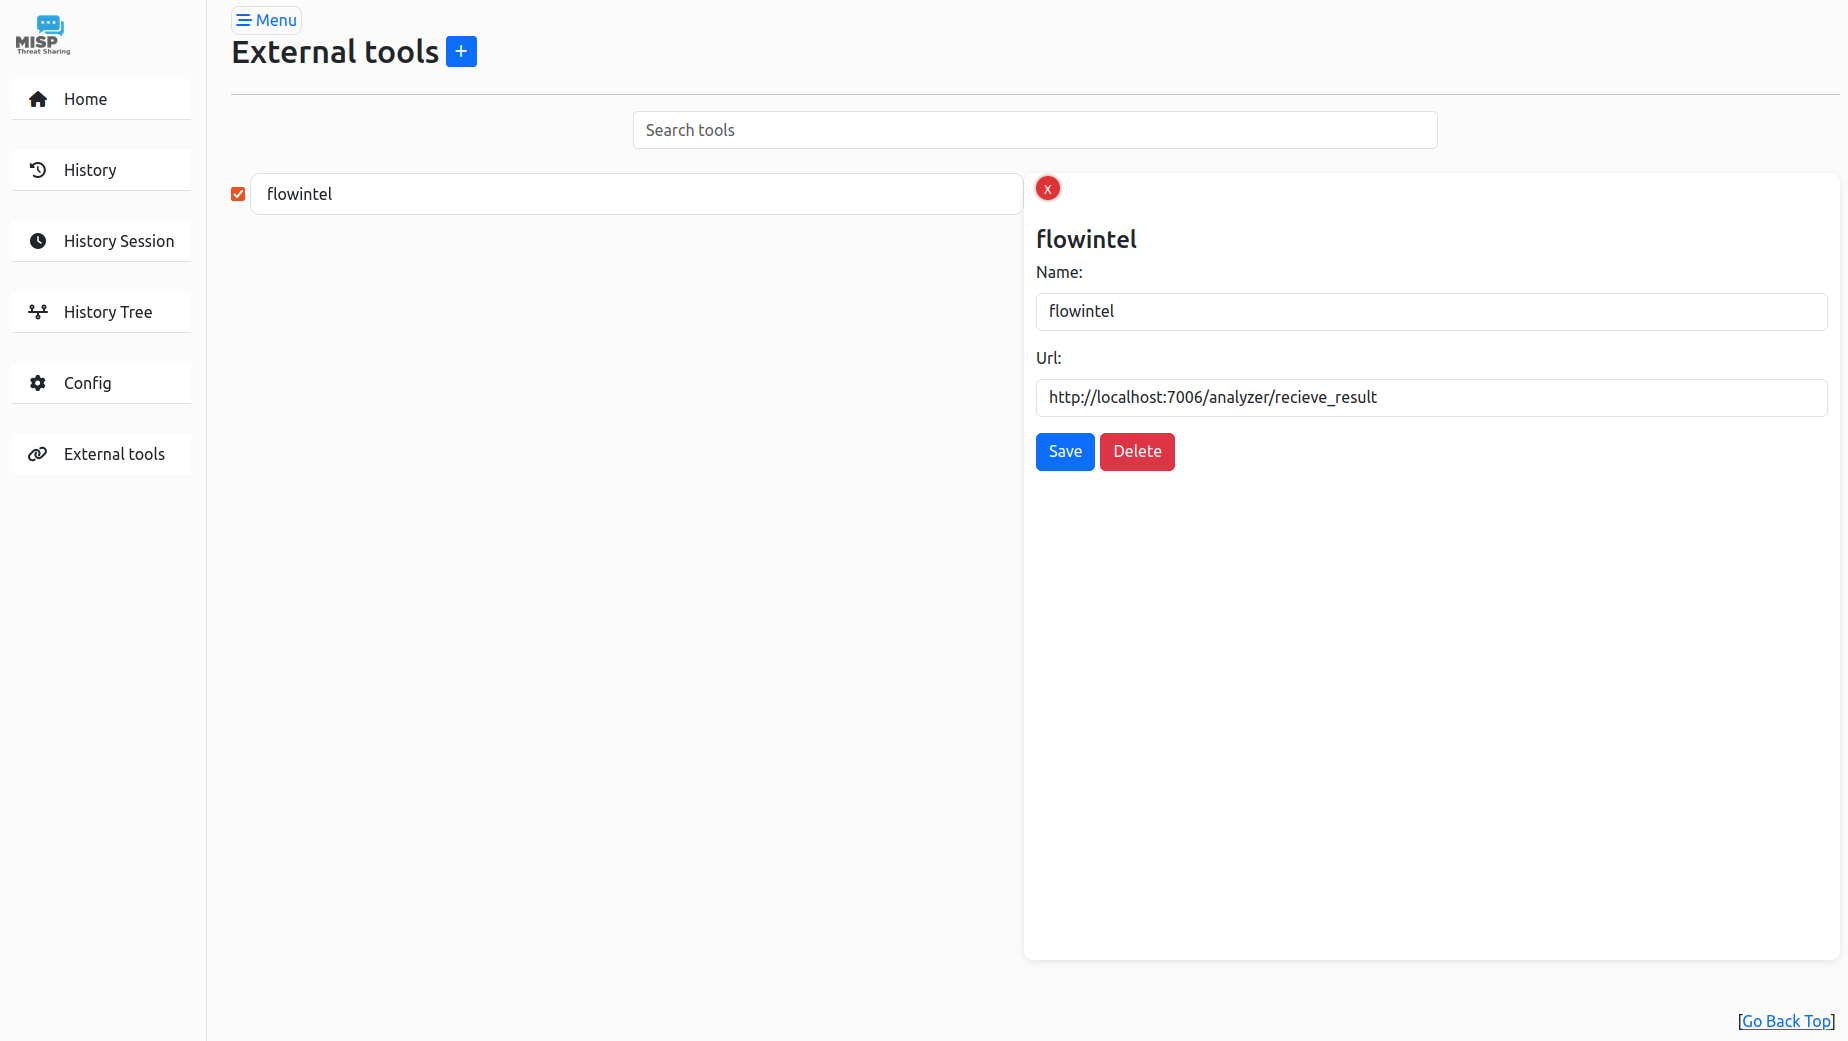
\includegraphics[scale=0.23]{screenshots/misp_module_external_tools.png}
\end{frame}

\begin{frame}[fragile]
    \frametitle{Future of the modules system}
    \begin{itemize}
        \item Enrichment on full events
        \item Move the modules to background processes with a messaging system
        \item Have a way to skip the results preview
        \begin{itemize}
            \item Preview can be very heavy
            \item Difficulty is dealing with uncertain results (without the user having final say)
        \end{itemize}
    \end{itemize}
\end{frame}

\begin{frame}[t,fragile] {Q\&A}

\includegraphics[scale=0.5]{misplogo.pdf}
\begin{itemize}
        \item \url{https://github.com/MISP/misp-modules}
        \item \url{https://github.com/MISP/}
        \item We welcome new modules and pull requests.
        \item MISP modules can be designed as standalone application.
\end{itemize}

\end{frame}
